\chapter{Proposed Solution}
\label{implementation}
\thispagestyle{plain}

\section{Overview}
\label{subsubsec:solution-overview}
After researching through the various proposals for solving different timetabling problems (e.g. ~\cite{Bajeh2001},~\cite{Chiarandini2006}) it became clear that although genetic algorithms (GA) are an appropriate method to solve this type problem, it also became clear that it’s not efficient in terms of time and computation effort needed to attain feasible solutions, when compared with other strategies such as tabu search or simulated annealing. In fact, the work submitted by Chiarandini et al. ~\cite{Chiarandini2006} proposes that the usage of meta-heuristic algorithms such as GA and Ant Colony Optimization (ACO) alone should be hybridized with local search procedures in order to achieve good results.\\
\\
With this in mind and since the ITC2007 rules ~\cite{McCollum2007} for evaluating the algorithms indicate that the solutions must be produced within a time limit, it became apparent that it would be more appropriate to explore a hybrid approach, in which:\\
\begin{itemize}
\item A GA is used to create the initial feasible solutions 
\item	A local search algorithm – i.e. Simulated Annealing - is applied over the results produced by the GA in order to improve the quality of solutions.
\end{itemize}

The general overview is depicted in Figure~\ref{fig:overviewProposedApproach}.\\
\begin{figure}[h!]
 \centering
   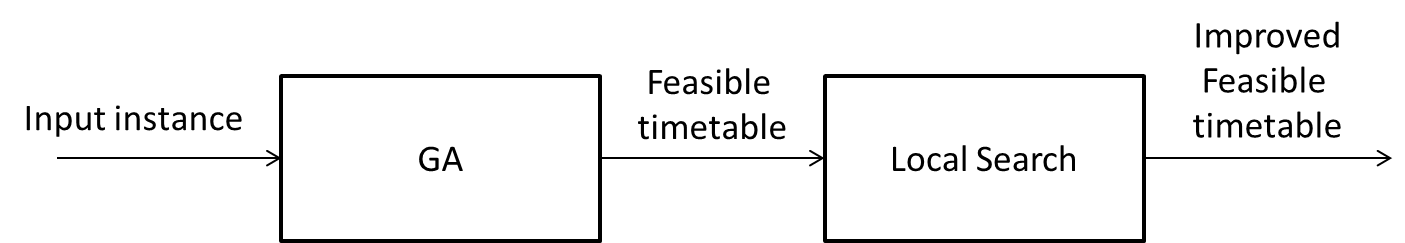
\includegraphics[width=12.5cm]{./images/figures/Fig1_OverviewProposedApproach.png}
   \caption{Overview of the proposed approach.}
   \label{fig:overviewProposedApproach}
\end{figure}\\
%%%%%%%%%%%%%%%
\section{First Phase - Genetic (Evolutionary) Algorithm}
\label{subsubsec:genetic-algorithm}
In the first stage, for the proposed genetic algorithm, only the hard constraints are considered, meaning that the fitness function used in this stage, will take into account only the violations of hard constraints, in an attempt to produce feasible timetables where all of these constraints are satisfied.\\
It’s expected that in the end of this first stage, the algorithm will have produced at least one feasible timetable and it will initiate the second stage if and only if a feasible timetable is found.\\ 
\\
Figure~\ref{fig:overviewProposedSteps} ilustrates the steps that will be executed by the algorithm.\\
\begin{figure}[h!]
 \centering
   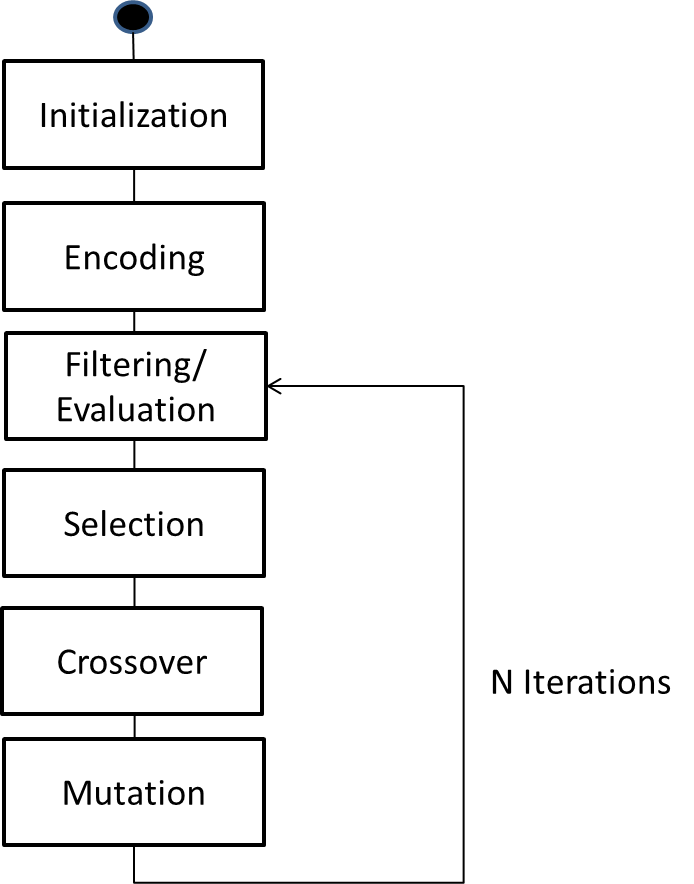
\includegraphics[width=7.05cm]{./images/figures/Fig2_OverviewSteps_GA.png}
   \caption{Overview of the steps of the proposed genetic algorithm.}
   \label{fig:overviewProposedSteps}
\end{figure}\\
The following subtopics present an overview of the implementation considerations that will be taken into account in each one of these steps.\\
%%%%%%%%%%%%%%%
\subsection{Initialization}
\label{subsubsubsec:ga-initialization}
The algorithm in the initialization step will create a population of chromosomes. In this stage we propose to use a sequential greedy heuristic as proposed by Lü et al. ~\cite{Lue2010} starting from an empty timetable, where assignments are constructed by inserting one appropriate lecture into the timetable at each time. At each step, two distinct operations are carried out: one is to select a still unassigned lecture of a course and the other is to determine a period-room pair for this lecture.\\
The algorithm does not place a course lecture in a timeslot which is not available for that course, and will attempt to satisfy this constraint satisfied in the next generations for as long as possible.  After the completion of the generation of the population, the resulting timetables will be encoded as chromosomes.\\
\\
\subsection{Encoding}
\label{subsubsubsec:ga-encoding}
The proposal for encoding the chromosomes that represent the timetables consists of using a 1 dimensional array of binary values, with a structure such as the one in Figure~\ref{fig:chromosomeRepresentation}.\\ 
\begin{figure}[h!]
 \centering
   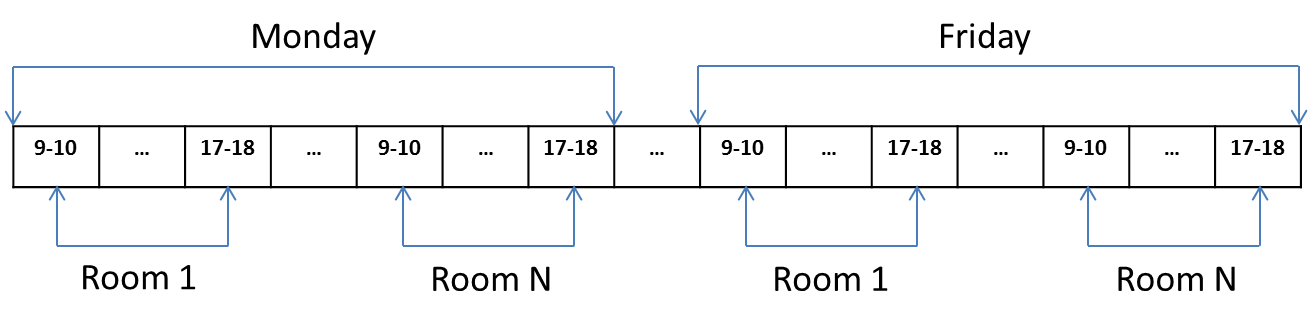
\includegraphics[width=15cm]{./images/figures/Fig3_ChromosomeRepresentation_GA.png}
   \caption{Chromosome representation.}
   \label{fig:chromosomeRepresentation}
\end{figure}\\
Each cell in the array represents a timeslot. A group of X adjacent timeslots represents one day of lectures that can be assigned in a single room. A group of Y adjacent room-timeslots represents the one day of lectures that can be allocated on that given day. Value 0 represents that the timeslot is available for allocation, 1 represents that it is already alocated.\\
The information regarding the lecturer, curriculum, etc. will be maintained on an associative array that will keep the information regarding the current allocated position in this array.\\
\subsection{Evaluation}
\label{subsubsubsec:ga-evaluation}
A fitness value is assigned to each timetable based on the number of violations of hard and soft constraints detected. In each generation the chromosomes are evaluated and then the chromosome pool is sorted. The evaluation process employs a fitness function to calculate the fitness of each timetable.\\
\subsection{Selection}
\label{subsubsubsec:ga-selection}
In the selection step, the fittest individual will be kept unchanged. The remaining individuals will subjected to a tournament selection method. In this method, K chromosomes are chosen from the population, and the ones with a greater fitness value will be selected to perform the crossover, and thus generate new offspring that will replace the K least fit individuals.\\
\subsection{Crossover}
\label{subsubsubsec:ga-selection}
During the implementation phase, experiments with different types of crossover operators – e.g. One-Point Crossover, Two-Point Crossover, N-Points Crossover – will be conducted in order to evaluate which one of these is more adequate to generate the offspring.\\
\subsection{Mutation}
\label{subsubsubsec:ga-mutation}
The mutation function randomly exchanges the values in every pair in a random number of location pairs of a timetable. The mutation rate is not fixed. In each generation the maximum and average fitness values will be calculated. If the two numbers are close enough to each other, the mutation rate value will be increased to avoid any chance of an early convergence.\\
\subsection{Repair Function}
\label{subsubsubsec:ga-repairfunction}
It is expected that the application of the crossover operator will produce non feasible solutions, possibly with worse fitness values than the K least fit individuals that were determined in the selection step. Therefore, instead of purging the K least fit individuals immediately after the crossover step, a new fitness evaluation will be performed over the new population along with the K least fit individuals. After this evaluation, the new K least fit individuals group will be purged, and a new iteration of the process will begin.\\
%%%%%%%%%%%%%%%
\section{Second Phase - Simulated Annealing Algorithm}
\label{subsubsec:genetic-algorithm}
Simulated annealing (SA) has been widely used to solve combinatorial optimization problems. It accepts the new solution when the objective value, which is determined by an objective function, is lower than or equals to the current one. There is a probability to accept worse quality solution using a probability acceptance function which controls the acceptance of the new solution. The current temperature is iteratively reduced according to the cooling schedule with a given cooling rate in each iteration or level until its temperature reaches final minimum temperature which is close to zero.\\ 
When the SA temperature becomes very low, the SA will exhibit a behavior similar to a descent heuristic (i.e. accepts only an improving solution) and therefore the search might be trapped in local optimum. To limit this effect, reheating will be used, in order to attempt to restart the search in another point in the search space.\\
The proposed SA algorithm involves: neighborhood structure, temperature, cooling schedule, termination criteria.
\begin{itemize}
\item Case I: The minimum temperature is close to zero 
\item Case II: Number of iterations reaches the limit
\item Case III: Timeout based on the ITC 2007 course timetabling track 3 stopping condition.
\end{itemize}
%%%%%%%%%%%%%%%
\section{General System Architecture Overview}
\label{subsubsec:solution-architecture-overview}
In this section we discuss the general system architecture that will be implemented. Figure~\ref{fig:systemArchitecture} illustrates the proposed architecture.\\
\begin{figure}[h!]
 \centering
   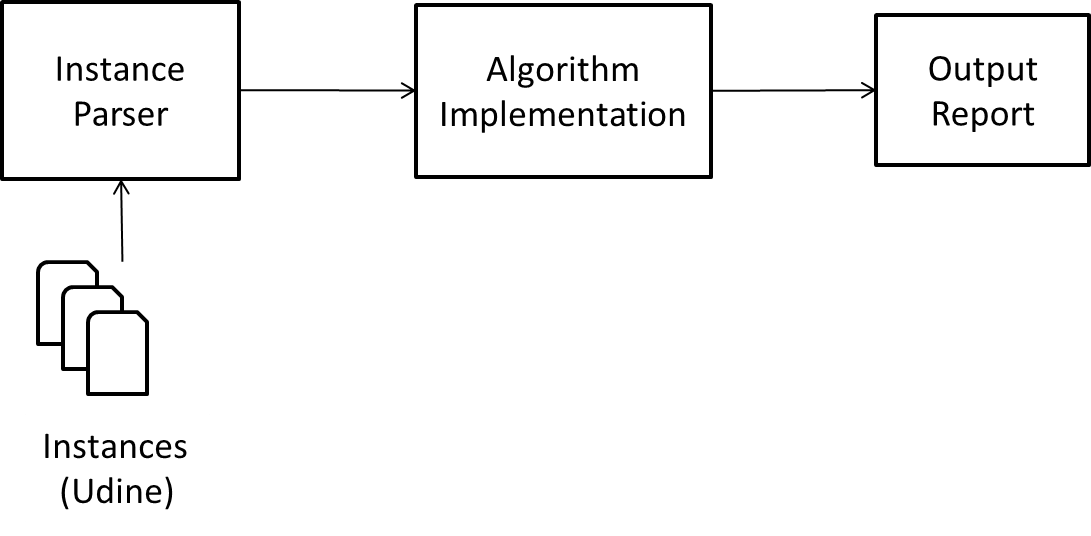
\includegraphics[width=15cm]{./images/figures/Fig4_SystemArchitecture.png}
   \caption{General System Architecture.}
   \label{fig:systemArchitecture}
\end{figure}\\
The instance parser is the component responsible for parsing the problem instances that were provided by the University of Udine for the ITC 2007 Track 3 competition. The instances will loaded in memory. After the instances are loaded, the implemented algorithms modules will be executed. After the completion of the execution, a report file will be generated with the information regarding the best solution and data regarding metrics (e.g. Time executed, CPU time, etc).\\
The system will be implemented as a normal Java console application. The motivation regarding the usage of Java for the implementation is the availability of third party components that can be useful in the data manipulation and visualization, which can benefit the analysis of the results.\\
As a general requirement, the application should be able to obtain configuration data that can be used to perform tuning of parameters used in the solver algorithms (e.g. the parameters used in the cooling schedule of simulated annealing algorithm).
%%%%%%%%%%%%%%%